\chapter{The CMS experiment at the LHC}\label{ch:cms}

\section{Introduction}\label{sec:cms_intro}
\noindent Located in the Swiss-French border, the European Council for Nuclear Research (CERN) is the largest scientific organization leading the particle physics research. About 13000 people in a broad range of fields including users, students, scientists, engineers among others, contribute to the data taking and analysis, with the goal of unveiling the secrets of the nature and revealing the fundamental structure of the universe. CERN is also the home of the Large Hadron Collider (LHC), the largest circular particle accelerator around the world, where protons (or heavy ions) traveling close to the speed of light, are made to collide. These collisions open a window to investigate how particles (and their constituents if they are composite) interact with each other, providing clues about the laws of the nature.

\noindent LHC can run in three modes depending on the particles being accelerated

\begin{itemize}
\item Proton-Proton collisions (pp) multiple physics experiments .
\item Lead-Lead collisions (Pb-Pb) Heavy ion experiments. 
\item Proton-Lead collisions (p-Pb).
\end{itemize}

\noindent Figure \ref{cern} show an overview of the CERN accelerating complex. There are several accelerating stages before the injection to the LHC ring. In the pp mode, after removing the electrons from hydrogen atoms in a bottle, protons are accelerated in the LINAC2 to 50 MeV and then injected into the proton synchrotron booster (BOOSTER) to reach 1.4 GeV in energy. The next boost is provided at the proton synchrotron (PS) up to 26 GeV, followed by the injection into the super proton synchrotron (SPS) where protons are accelerated to 450 GeV. Finally, protons are injected into the LHC where they are accelerated to the target energy of 6.5 TeV. In the Pb-Pb mode, the Lead ions are first accelerated in the LINAC3 and then passed as long pulses to the Low energy ion ring (LIER) to be converted into short and dense bunches, each containing $7\times10^7$ lead ions. LEIR accelerate the bunches from 4.2 MeV to 72 MeV. The ions are then passed to the PS to follow the rest of acceleration process up to 2.8TeV/n en the LHC ring. 

\begin{figure}[!h]
  \centering
  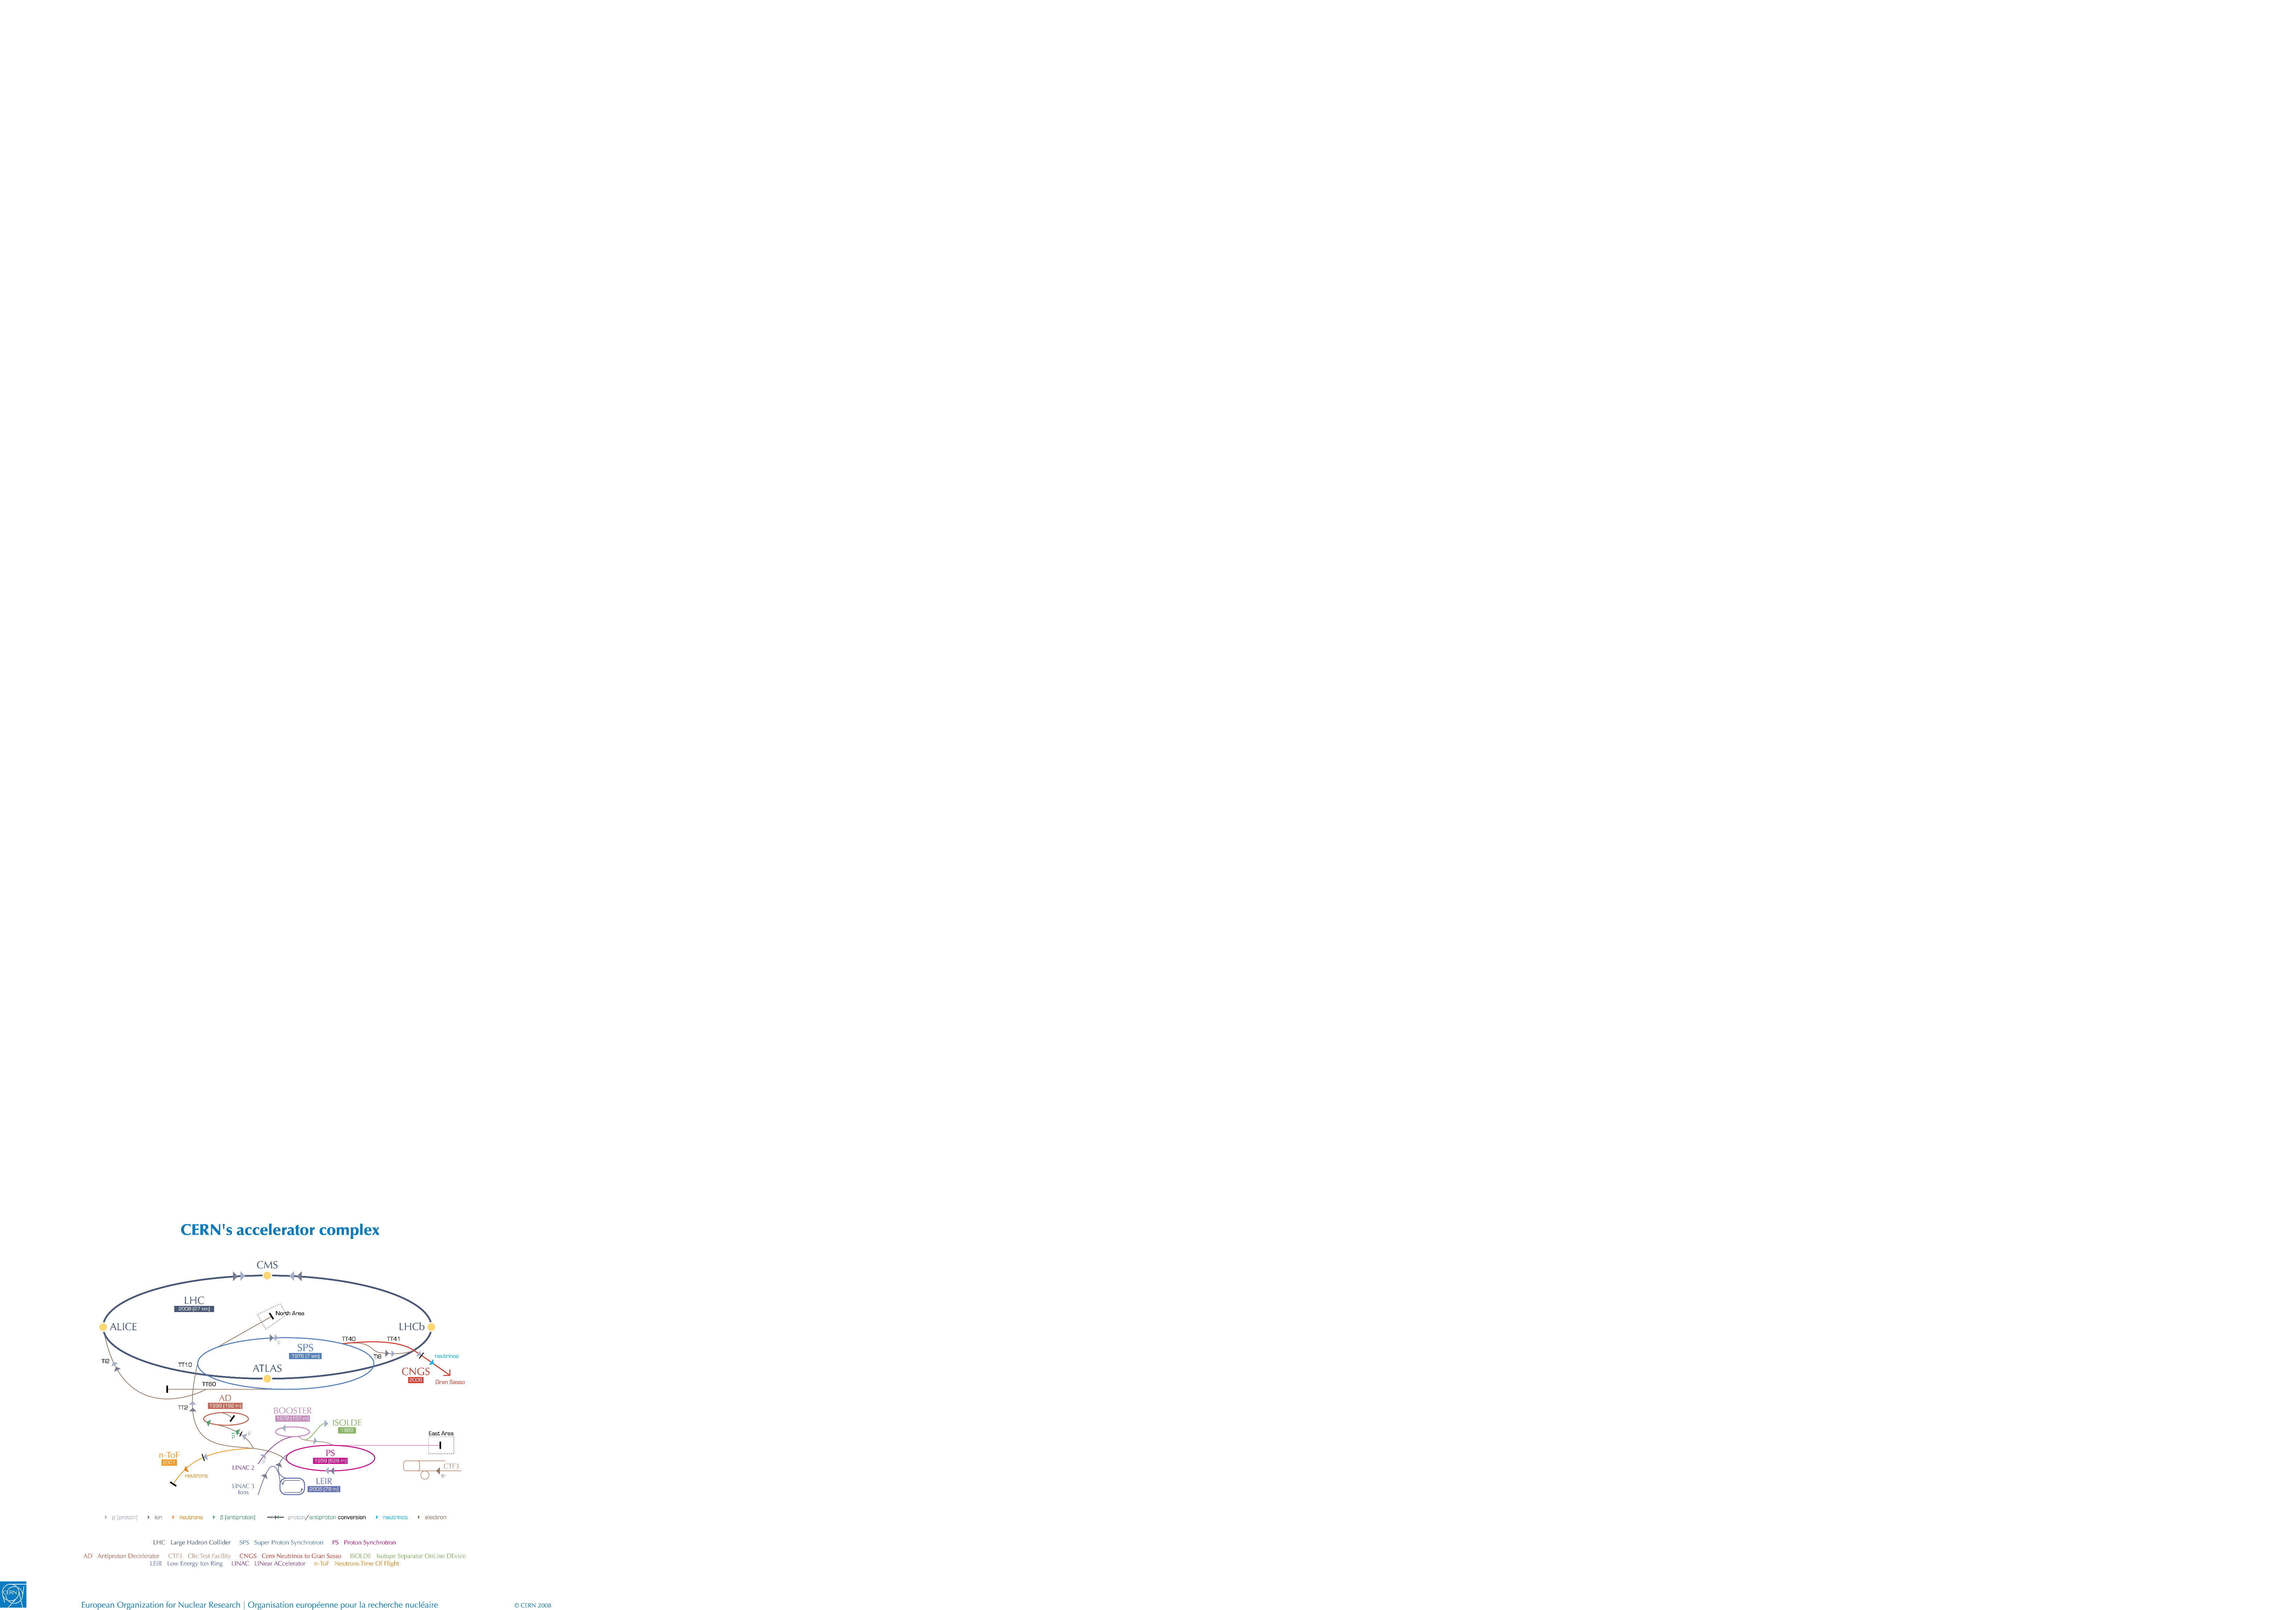
\includegraphics[width=\textwidth]{cern}
  \caption {ref. C.Lefevre, ``The CERN accelerator complex,'' (2008). CERN-DI-0812015.  }\label{cern}
\end{figure}


\section{The LHC}

The LHC is a 27 km ring composed of superconducting magnets and accelerating structures (among other components) which boost the particles traveling inside it. It is installed in the same tunnel where the large Electron-Positron (LEP) collider was located, taking advantage of the existing infraestructure as shown in Figure \ref{lep}. Two particle beams travel counter-rotating in two separated beam pipes kept at ultra high vacuum. In 2008, the first set of collisions involved protons with center-of-mass energy of 7 TeV after which the energy was increased to 8 TeV in 2012 and to 13 TeV in 2015. 

\begin{figure}[!h]
\centering
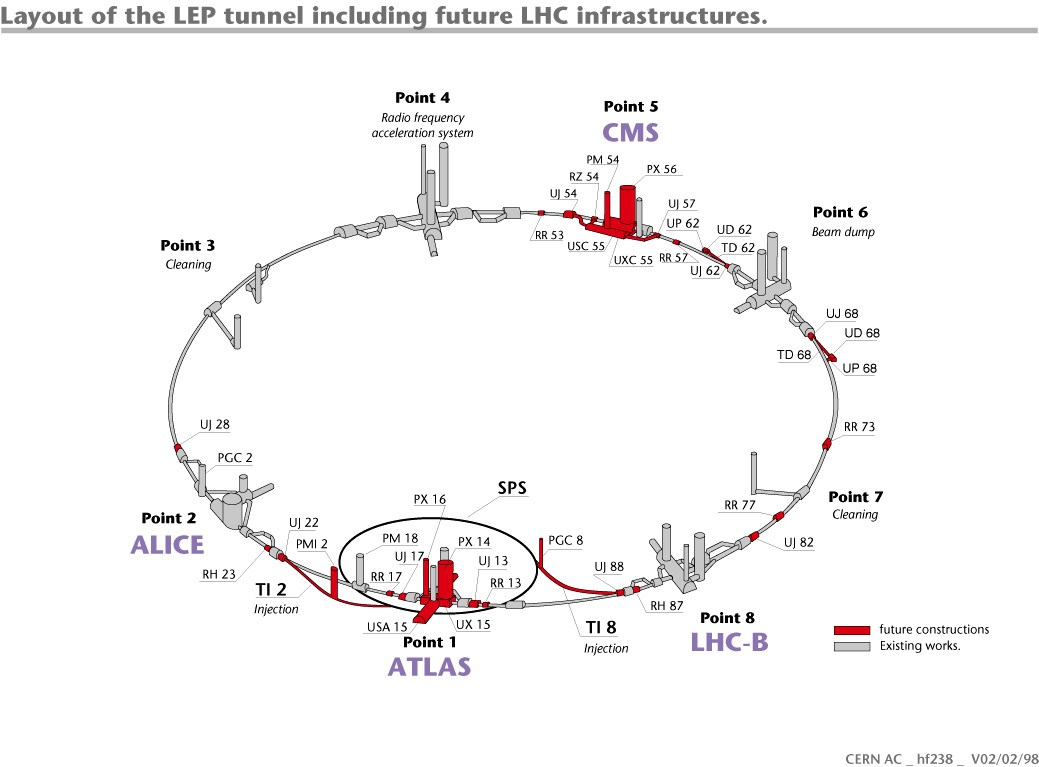
\includegraphics[width=\textwidth]{lep}
\caption {ref. J.-L. Caron , ``Layout of the LEP tunnel including future LHC infrastructures.. L'ensemble du tunnel LEP avec les futures infrastructures LHC.'',  https://cds.cern.ch/record/841542  (Nov, 1993). AC Collection. Legacy of AC. Pictures from 1992 to 2002.. }\label{lep}
\end{figure}

In order to keep the protons in the circular trajectory carrying that amount of energy, strong magnetic fields are needed, bringing the superconductivity into scene. The superconducting dipole magnets used in LHC are made of a NbTi alloy, capable of transporting currents of about $12000$ A when cooled at a temperature below 2K by using liquid helium; that current generates a magnetic fields of 8.3 T. Figure \ref{lhcdipole} shows the transverse view of the LHC dipole magnets. Additionally, quadrupole magnets are used to focus the beam and some other magnetic multipoles are used to correct effects generated by the interaction among protons in the beam as well as interactions within the beam pipe.

\begin{figure}[!h]
\centering
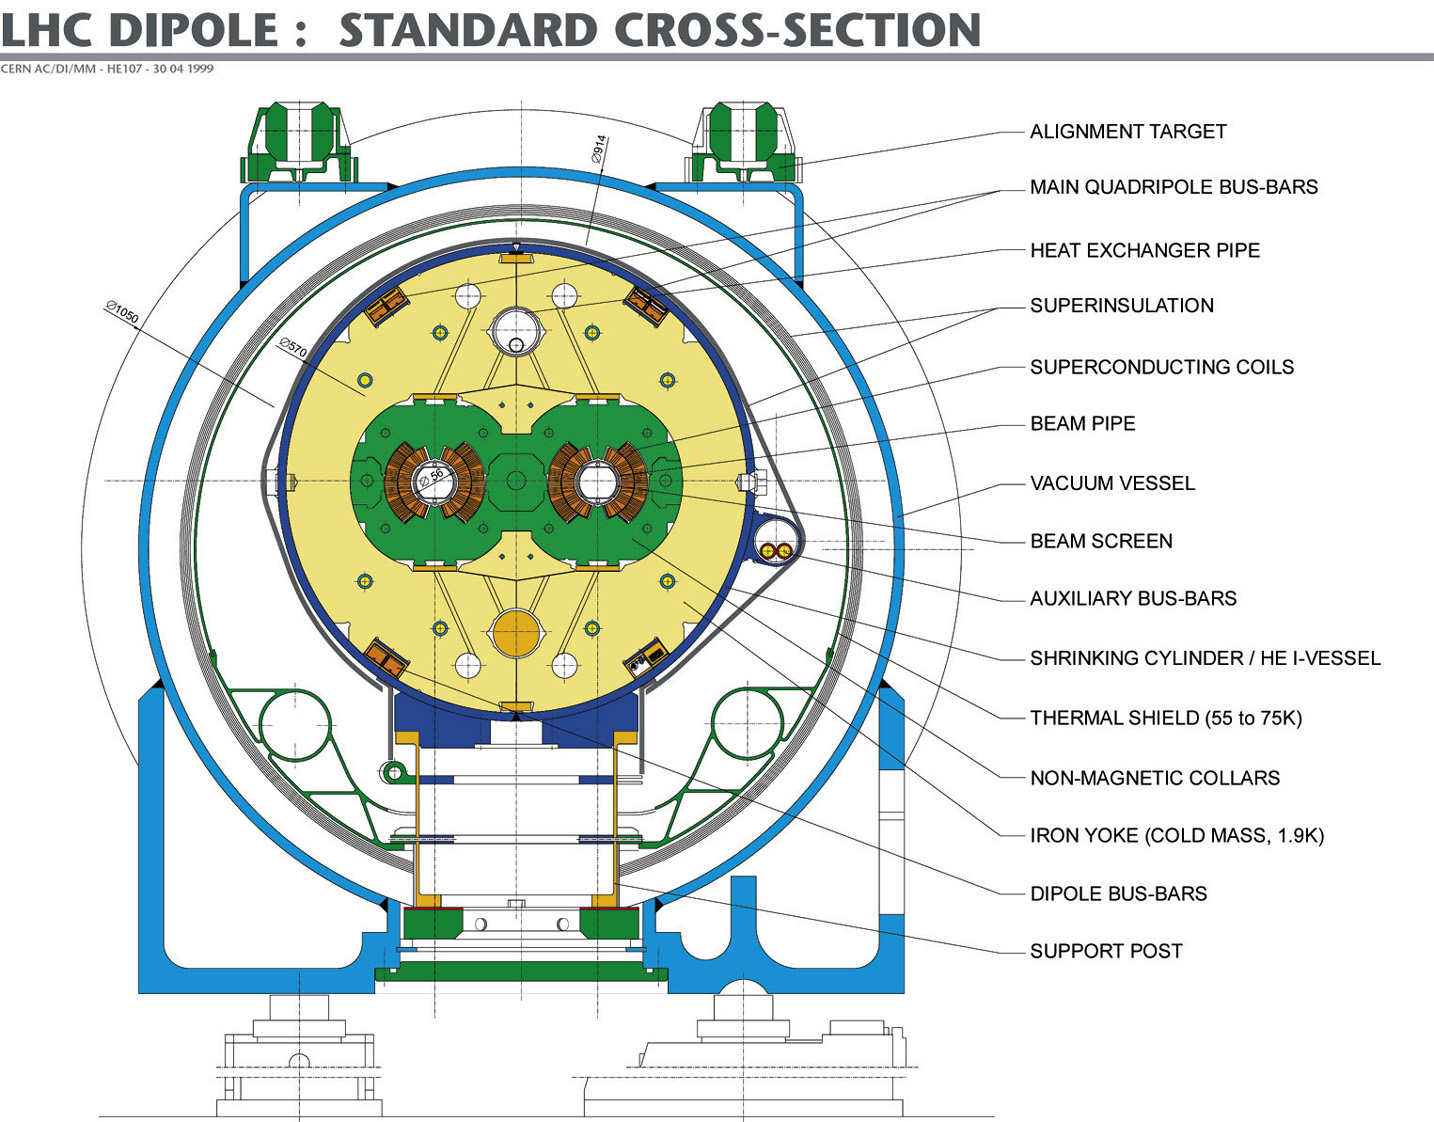
\includegraphics[width=0.7\textwidth]{lhcdipole}
\caption {ref. ACTeam, ``Diagram of an LHC dipole magnet. Sch\'ema d'un aimant dip\^ole du LHC,'' (1999). CERN-DI-9906025. }\label{lhcdipole}
\end{figure}

\noindent Regarding to the longitudinal acceleration of the protons, a system of 16 radio-frecuency cavities (RF) (8 per beam) is used to accelerate protons. Inside the cavities, the electromagnetic waves become resonant transfering the maximum energy to the particle flight through it. Cavities are cooled at 4.5 K. On LHC the RF oscillation frecuency is 400MHz and the protons are carefully timed so additionally to the acceleration effect the bunch structure of the beam is preserved. The Beam is made of 2808 ``bunches'' which are packages of $1.15 \times 10^11$ protons \ref{http://iopscience.iop.org/article/10.1088/1748-0221/3/08/S08001/pdf}. If LHC is at full energy, protons with the right energy does not feel any accelerating force but those with a different energy will be accelerated or decelerated to keep them in the bunch. The paths followed by particles during the acceleration process are shown in Figure \ref{cern}.


%% \begin{figure}[!h]
%% \centering
%% 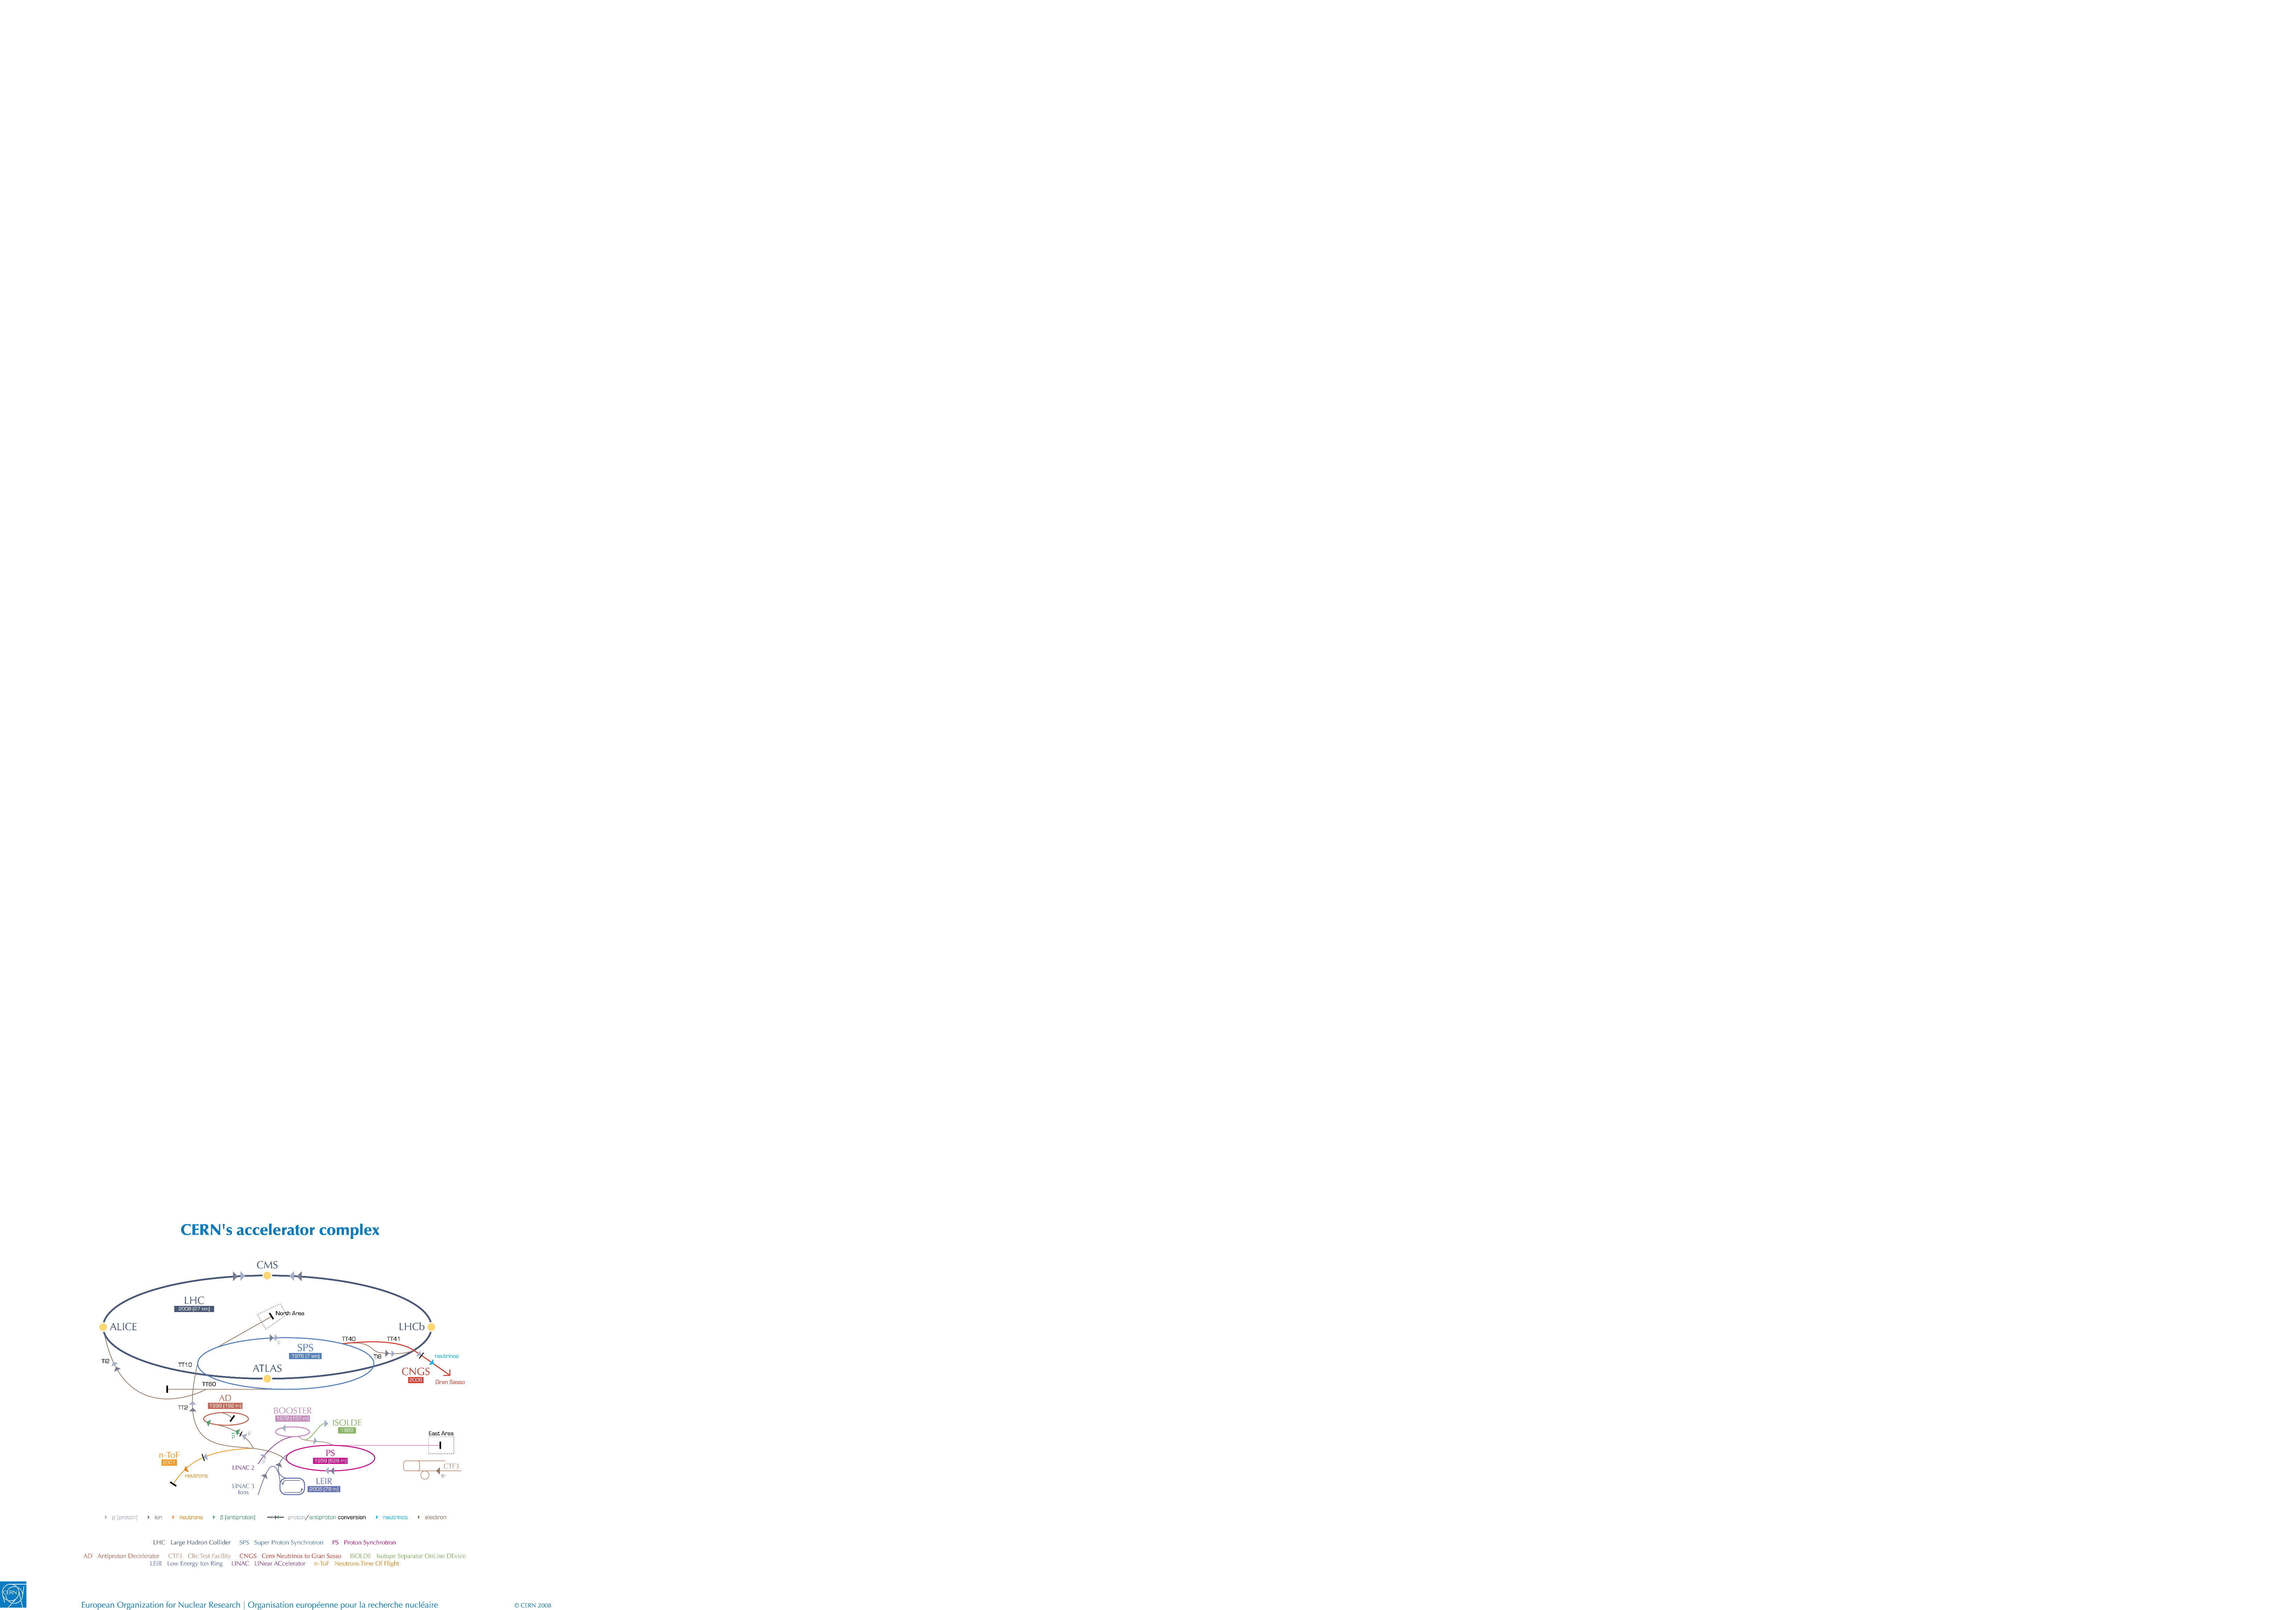
\includegraphics[scale=0.25]{cern}
%% \caption {C. Lefevre, ``The CERN accelerator complex. Complexe des acc\'el\'erateurs du CERN'', CERN-DI-0812015, https://cds.cern.ch/record/1260465, December, 2008.. }\label{cern}
%% \end{figure}


Once the beams reach the desired energy, they are brought to cross each other producing proton-proton collisions. The bunch crossing happens in precise places where the LHC experiments are located. As seen in Figure \ref{lep}, it was needed to build the caverns for CMS and ATLAS as well as some additional facilities, but most of the initial LEP infrastructure has been used to allocate additional collision points. The highest luminosity is delivered at the CMS (point 5) and ATLAS (point 1) experiments, which are general purpose experiments, enabled to explore physics in any of the collision modes. LHCb (point 8) experiment is optimized to explore B-physics, while ALICE (point 2) is optimized for heavy ion collisions researches; TOTEM (point 5) and LHCf (point 1) are dedicated to forward physics studies and MoEDAL (point 8) is intended for monopoles or massive pseudo stable particles studies.


\section{The CMS experiment}

The Compact Muon Solenoid (CMS) is a general purpose detector designed to conduct research in a wide range of physics from standard model to new physics like extra dimensions and dark matter. Located at the point 5 in the LHC layout as shown in Figure \ref{lep}, CMS is composed by several detection systems distributed in a cylindrical structure where the main feature is a solenoid magnet made of superconducting cable capable to generate a 3.8 T magnetic field. In total, CMS weight about 14000 tons in a very compact 21.6 m long and 14.6 m diameter cylinder (include areference for CMS TDR). It was built in 15 separated sections at the ground level and lowered to the cavern individually to be assembled. Figure \ref{cms} show the layout of the CMS detector (CMS TDR).          

\begin{figure}[!h]
  \centering
  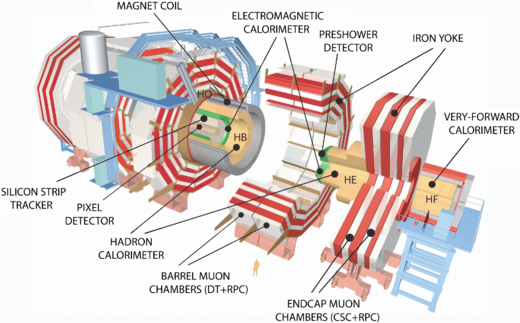
\includegraphics[width=\textwidth]{cms}
  \caption {ref: CMS Collaboration, ``Detector Drawings'', CMS-PHO-GEN-2012-002, http://cds.cern.ch/record/1433717, 2012. }\label{cms}
\end{figure}

